\documentclass{article}
\usepackage[a4paper]{geometry}
\usepackage[utf8]{inputenc}

\usepackage{graphicx}
\graphicspath{ {./images_P2/imatges_informe/} }


\title{Informe pràctica 2\\Visió Artificial}
\author{Jordi Olivares Provencio\\Christian José Soler}

\begin{document}

\maketitle

\begin{enumerate}

 \item \textbf{Procesamiento de imágenes con diferentes escalas y filtros 
de suavización}

 \begin{enumerate}

 \item \textit{Observar  cómo  desaparecen  los  detalles  de  la  imagen  cuando  se  re-escala 
(aumentando o reduciendo) el  tamaño de la imagen. ¿Cambia el histograma de 
las  dos imágenes  (la  original  y la  re-escalada)?  ¿Qué  pasa  con la  reducción  del 
tamaño de la imagen original? ¿Se pierden los detalles de la imagen re-escalada? 
¿El histograma cambia significativamente? }
 
 A simple vista, no se pierden detalles, pero en el histograma se ve que hay diferencias sutiles entre las dos imágenes (original y reescalada). 

  \begin{center}
 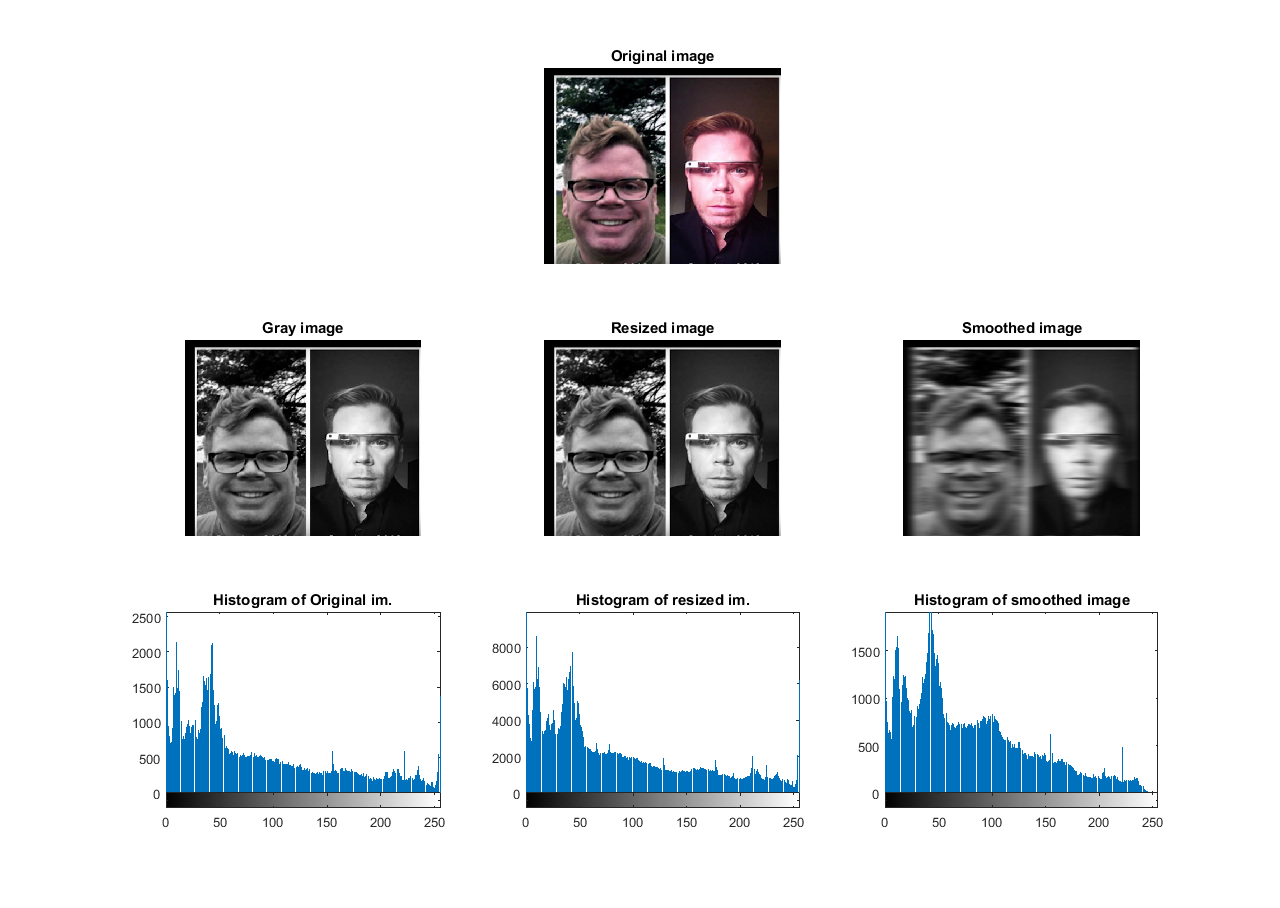
\includegraphics[width=0.8\textwidth]{1a.png}
 \end{center}

 \item \textit{Repetir la suavización varias veces para eliminar la línea del medio. ¿Cuántas iteraciones hace falta para eliminar la línea?}

 30 iteraciones son suficientes.

 \item \textit{Suavizar  con  una  máscara  vertical.  ¿Cuál  es  la  diferencia  en  la  imagen  filtrada 
aplicando  máscaras  horizontales  y  verticales? Nota: Para  visualizar  los 
diferentes resultados podéis cambiar los parámetros del subplot.}

 En el filtro horizontal se ve como si la imagen estuviera en movimiento horizontal y en el filtro vertical se ve como si la imagen estuviera en movimiento vertical.

  \begin{center}
 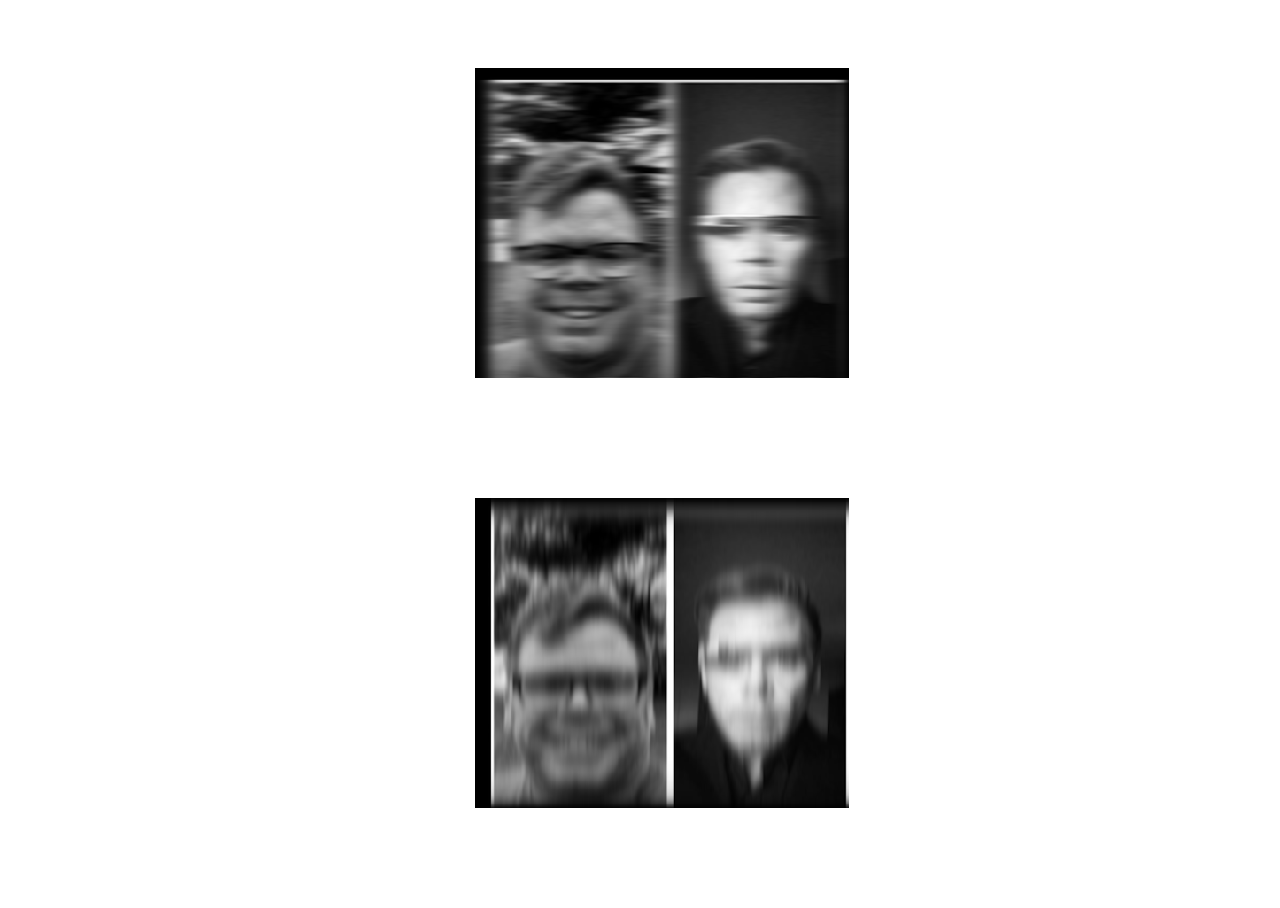
\includegraphics[width=0.8\textwidth]{1c.png}
 \end{center} 
 
 \item \textit{Seleccionar  una  de  las  imágenes  de  “images.zip” y repetir a)-c).  Aplicar 
diferentes tamaños de filtros y comentar los resultados.  Nota: Para ver mejor el 
efecto, escoger alguna imagen con textura}

  Podemos observar los mismos resultados que con la imagen original. Presentamos los histogramas y la imágen pasado por filtro vertical y horizontal. Nuestras conclusiones son las mismas de antes
 
   \begin{center}
 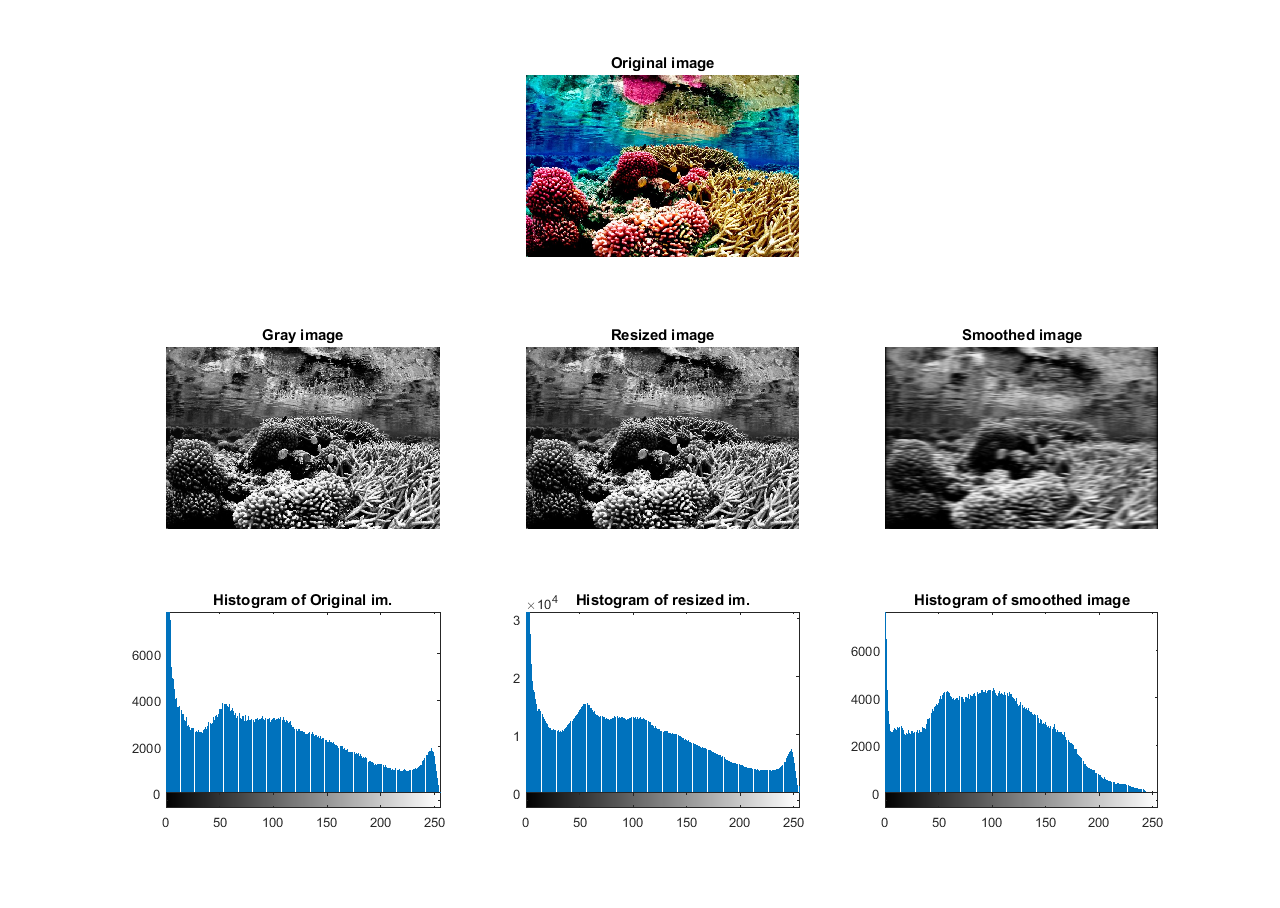
\includegraphics[width=0.8\textwidth]{1d(a).png}
 \end{center}
 
 
   \begin{center}
 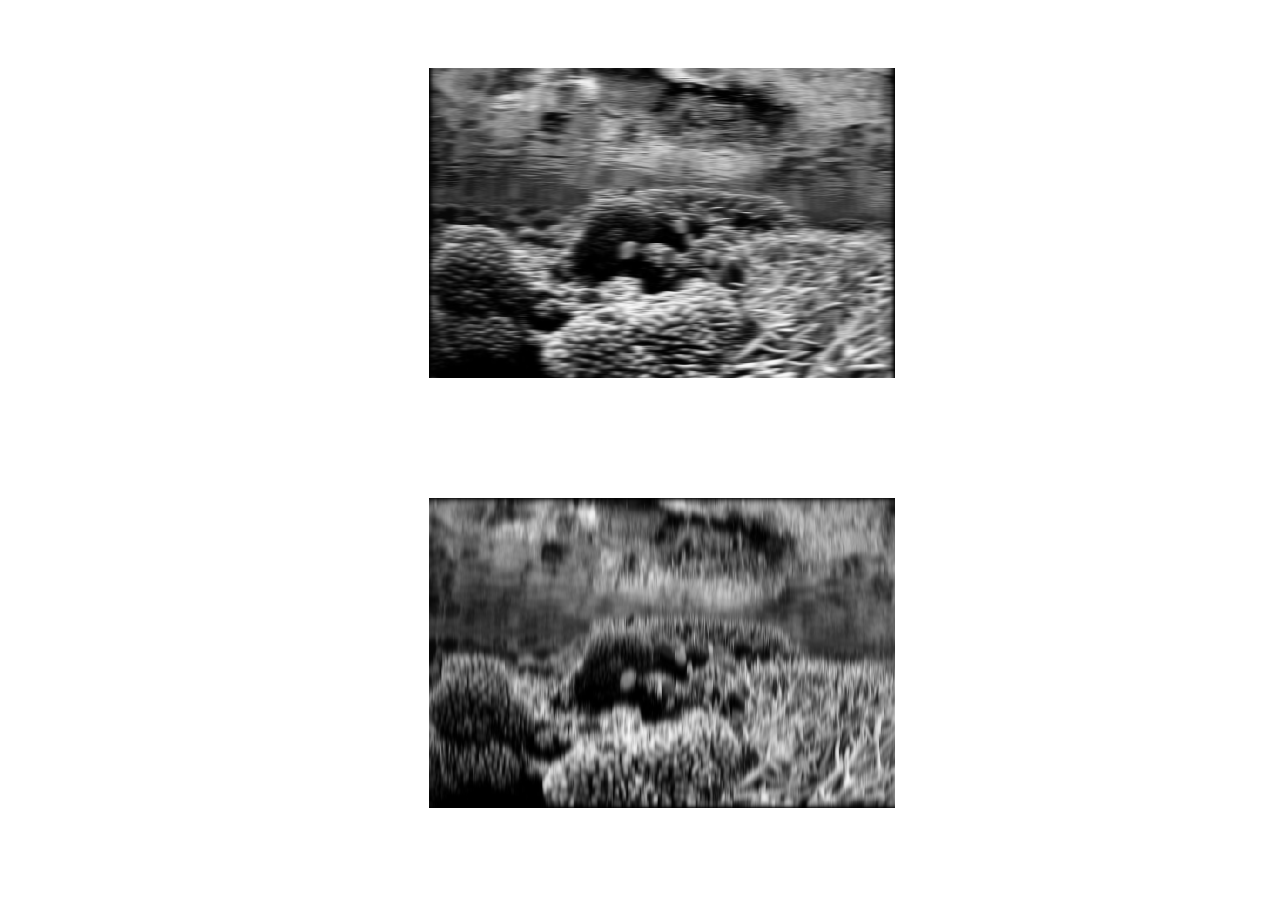
\includegraphics[width=0.8\textwidth]{1d(c).png}
 \end{center}
 
 \item \textit{Definir  una  máscara 2D.  Comentar  cómo  el  tamaño  de  la  máscara  afecta el 
resultado final del filtraje. }
 
 Hemos definido nuestra máscara como una matriz 10x10 de 1's normalizado.
 
 Probamos con otros tamaños nxn también y cuánto mayor es n, más borrosa se ve la imagen.
 
 
 \item \textit{¿Se  puede  aplicar  el  filtro  sobre  la  imagen  en  color?  ¿Se  puede  visualizar  el 
histograma de la imagen suavizada en color? ¿Qué tipo debe ser la imagen antes 
de aplicar la convolución y por qué?}
 
 Sí, se puede aplicar el filtro si se aplica canal por canal.
 
 Se puede visualizar el histograma, pero se ha de hacer canal por canal y con colores diferentes se puede superponer en el mismo histograma.
 
 La imagen debe estar en escala de grises antes de aplicar la convolución, porque está definida sobre números reales no sobre vectores (imagenes con varios canales de color)
 
 
 \newpage
 \item \textit{¿Cuál es la diferencia usando las siguientes máscaras: }
 
 [[1 1 1 1 1], [1, 1, 1, 1, 1]]  
  
  \begin{center}
 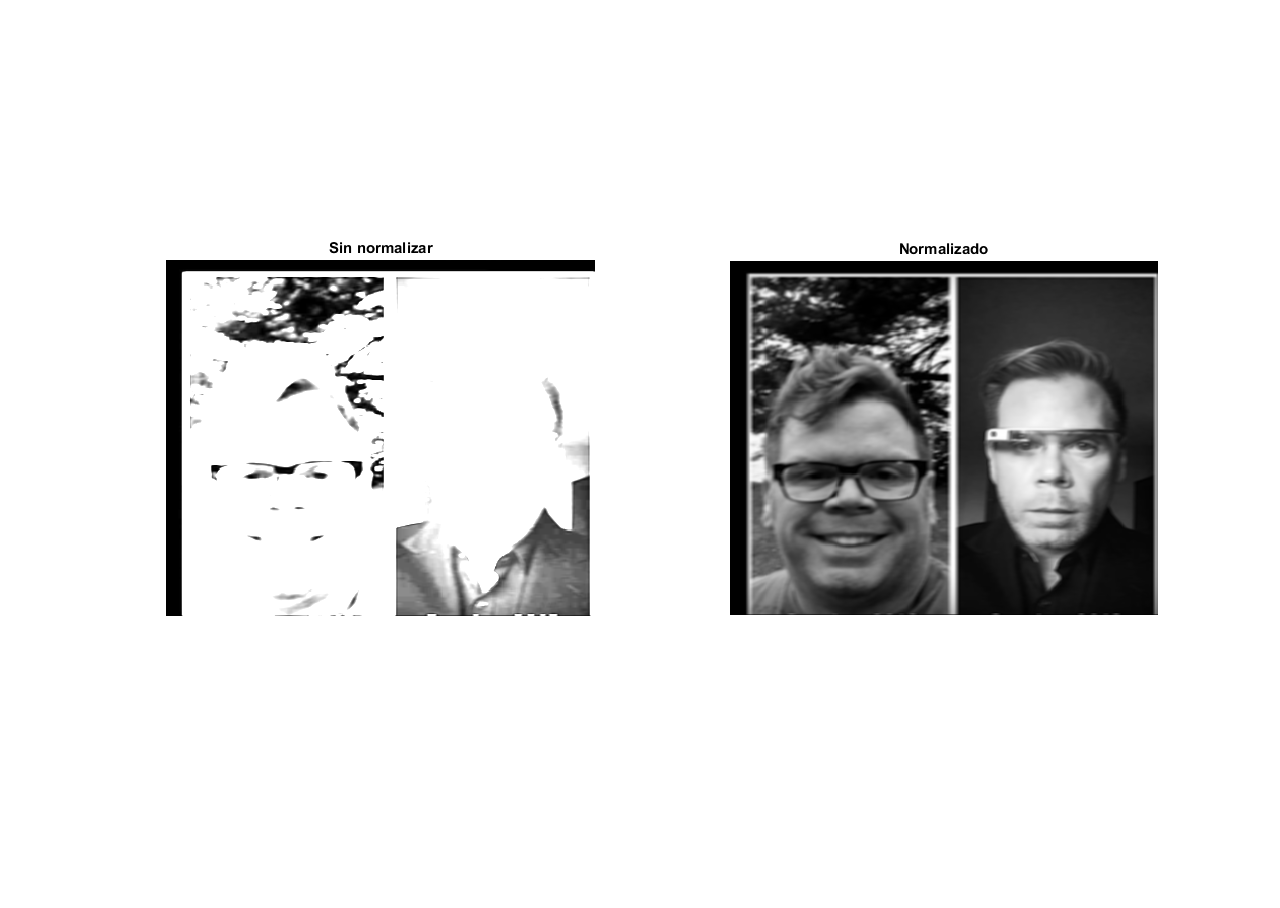
\includegraphics[width=0.8\textwidth]{1g(a).png}
 \end{center}  
  
  [[1 1 1 1 1]; [1 1 1 1 1]; [1 1 1 1 1]; [1 1 1 1 1]; [1 1 1 1 1]]
  
  \begin{center}
  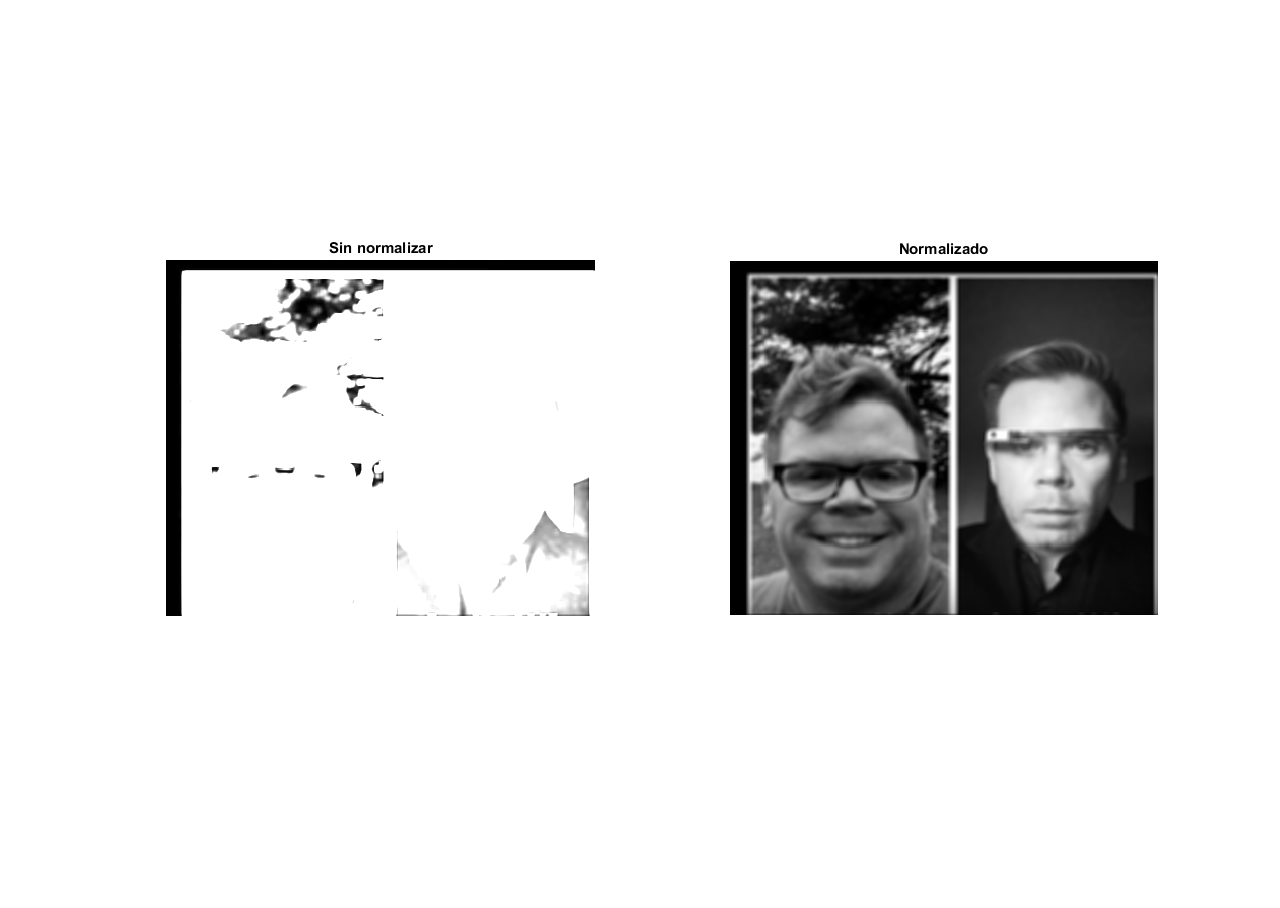
\includegraphics[width=0.8\textwidth]{1g(b).png}
  \end{center}
  
 \item \textit{¿Qué  pasa  si  no  normalizamos  la  máscara?  Aplica  varias  veces  la  convolución 
sobre la imagen con el fin de observar el efecto de suavizado mejor. }

 Se ve toda la imagen muy blanca, porque suma todas las intensidades y eso se dispara muy rápido. En el apartado (g) se ve el resultado sin normalizar también.

 \end{enumerate}

\newpage

 \item \textbf{Procesamiento de imágenes con filtros ponderados y filtres 
no lineales}

 \begin{enumerate}
 \item \textit{Generar  el  kernel  (núcleo)  de  la  Gaussiana  con  el  comando  de  Matlab  y  aplicar  la 
convolución  sobre alguna  de las imágenes seleccionadas para el Ejercicio  2.1.  Repetir 
100 veces la suavización para ver mejor el efecto. Comparar con la suavización con filtro 
de  la  media. Utilizar  diferentes  valores  de  sigma  y  comentar  su  efecto.  ¿Qué  valor  de 
sigma consideráis más adecuado para suavizar los detalles de esa imagen en concreto, y 
quedarse con los objetos y estructuras principales?}

  Imágenes con sigma = 0.4, 0.5, 1 respectivamente. Encontramos mejor el 0.4
  
 \begin{center}
 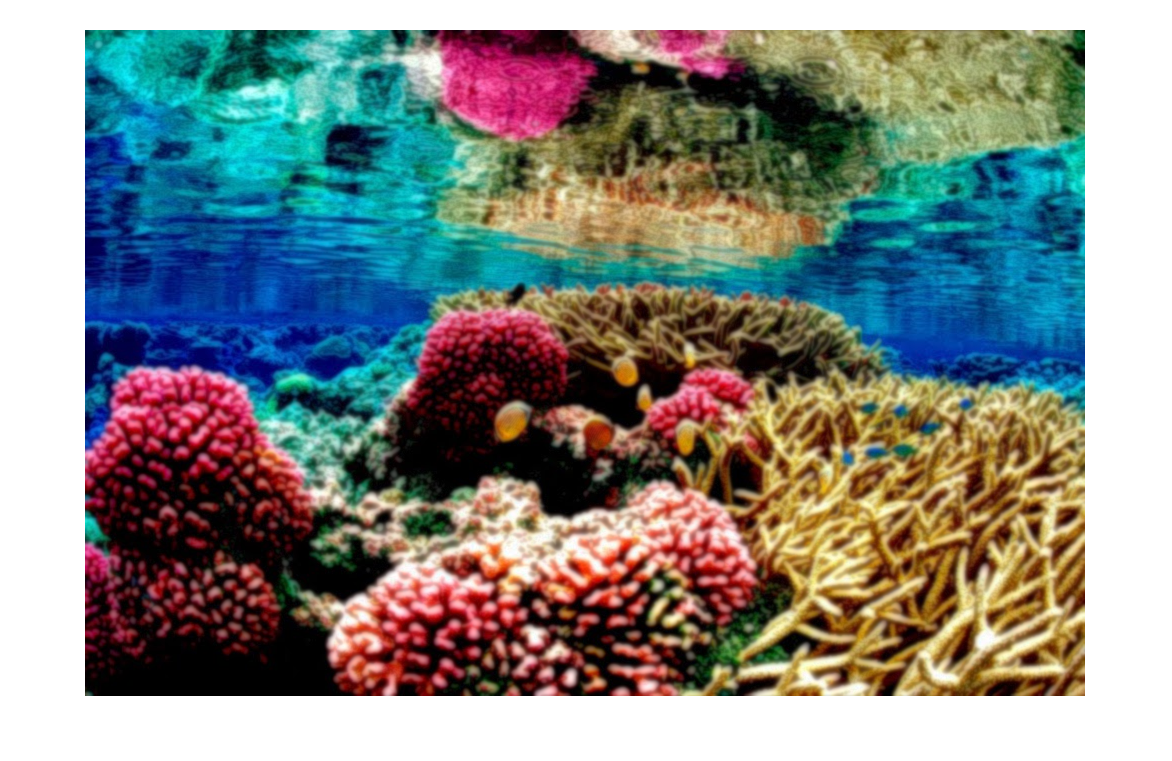
\includegraphics[width=0.6\textwidth]{2a(gaussian_04).png}
 \end{center}
 
 \begin{center}
 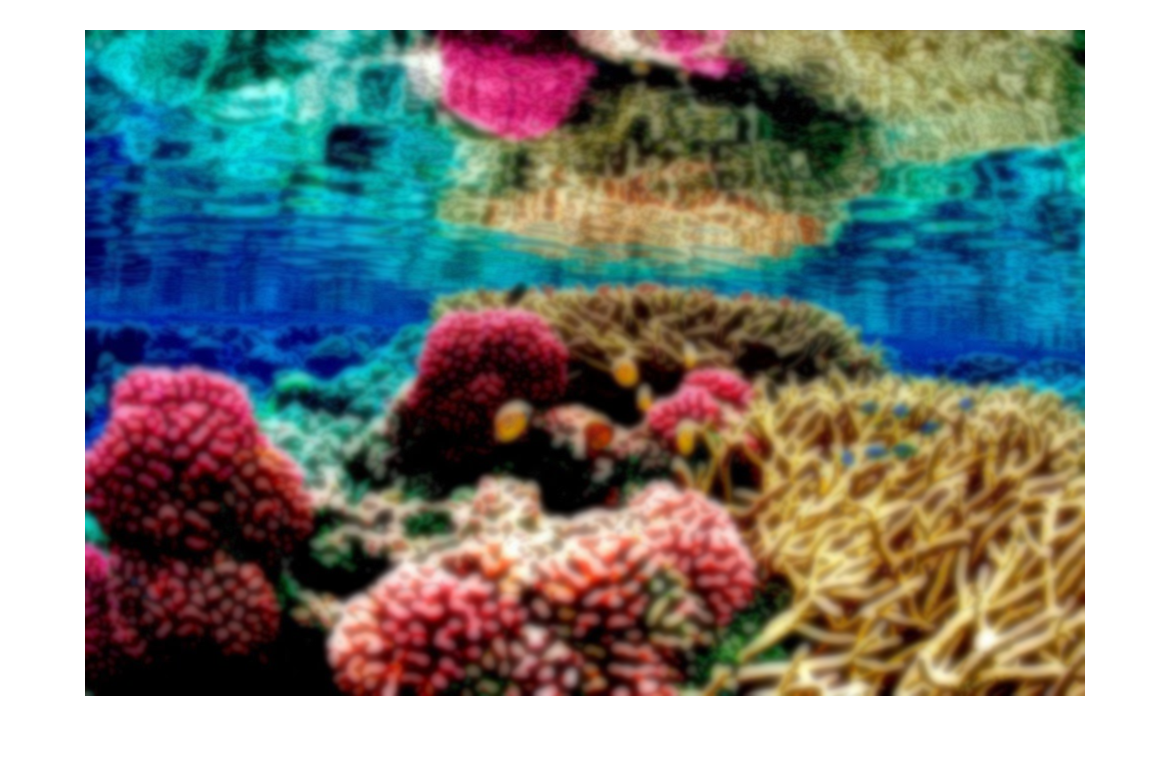
\includegraphics[width=0.6\textwidth]{2a(gaussian_05).png}
 \end{center}
 
 \begin{center}
 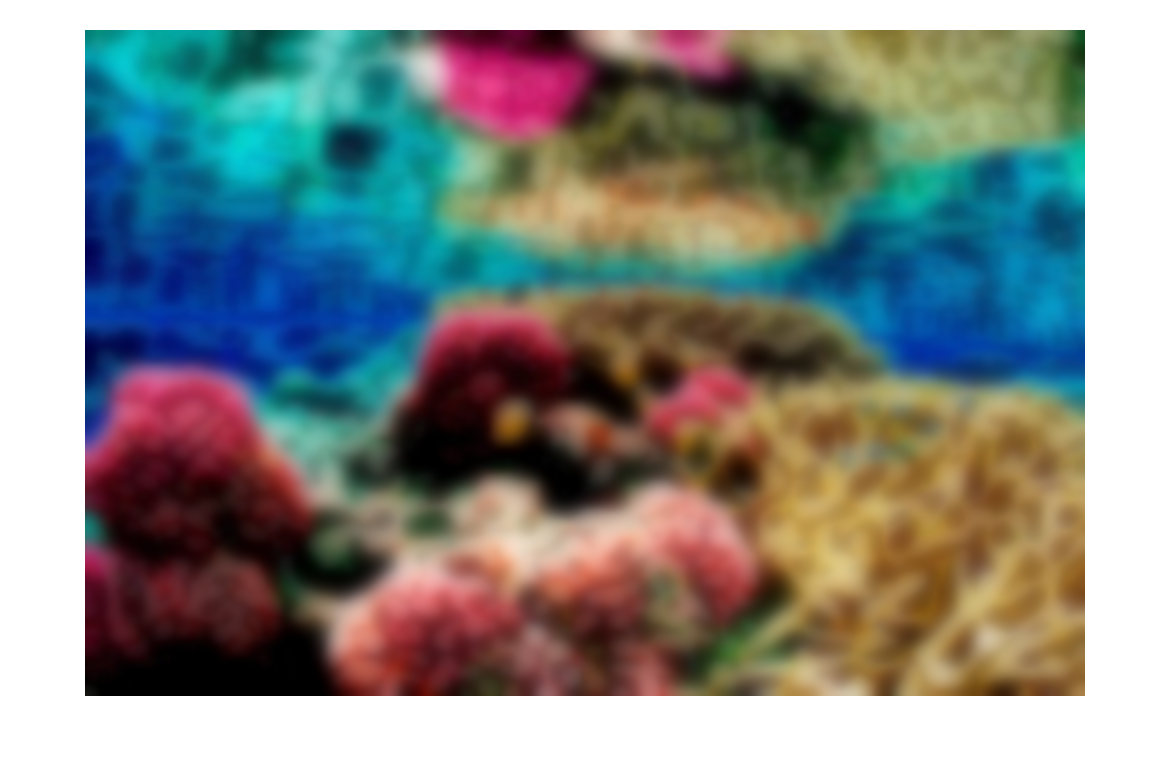
\includegraphics[width=0.6\textwidth]{2a(gaussian_1).png}
 \end{center} 

 El filtro de la media. Consideramos que el gaussiano con sigma=0.4 es mucho mejor
 
 \begin{center}
 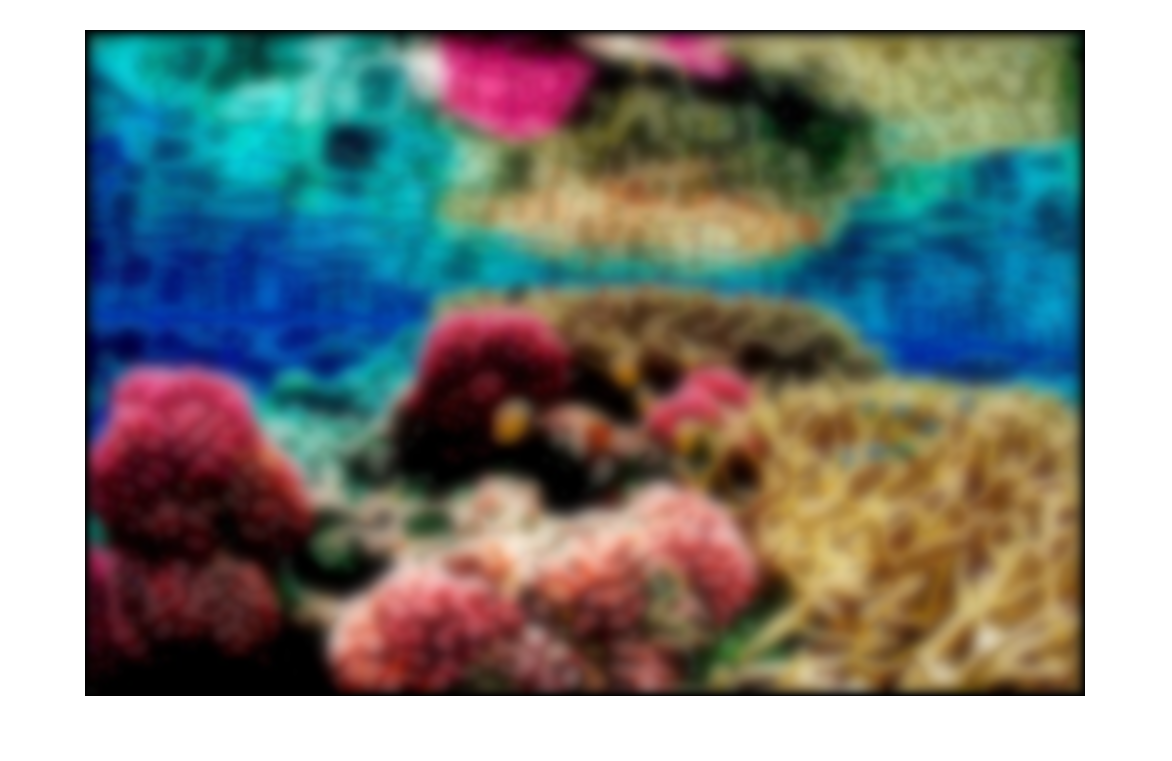
\includegraphics[width=0.6\textwidth]{2a(average).png}
 \end{center} 

 
 \newpage
 \item \textit{Proponer un  filtro alternativo al  filtro de la media que permite eliminar la línea del 
medio de la imagen ‘face.png’ aplicando el filtro una única vez. Restar la imagen original 
de la suavizada con el  fin de ilustrar la diferencia entre ellas  (ten en cuenta que algún 
píxel puede quedar en negativo).}

  Nuestro filtro es gausiano con sigma=10:

 \begin{center}
 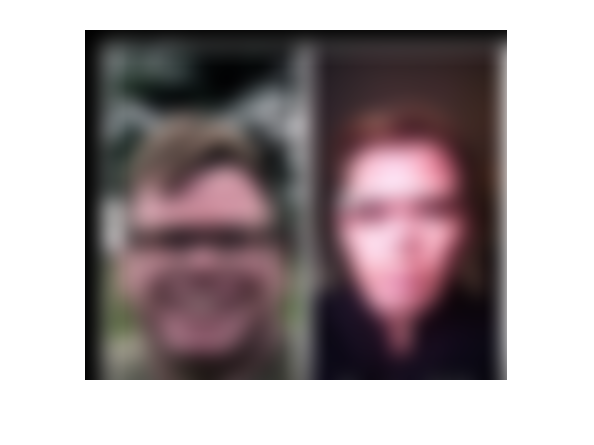
\includegraphics[width=0.6\textwidth]{2b.png}
 \end{center}

 Mostramos la imagen restada:
 
 \begin{center}
 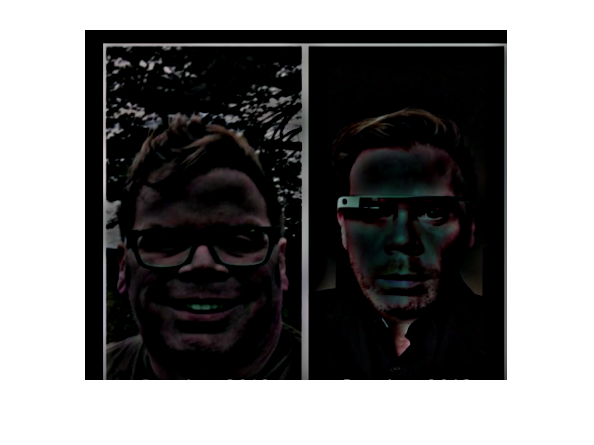
\includegraphics[width=0.6\textwidth]{2b(restados).png}
 \end{center}
 
 \end{enumerate}

\newpage

 \item \textbf{Determinar los contornos óptimos }

 \begin{enumerate}
 \item \textit{Leer  la  imagen  ‘logo.png’ y  encontrar  sus  contornos (¿Cuál  es  el  comando  en 
Matlab?)}

 El comando es imcontour

 \item \textit{Aplicar  los  diferentes  operadores  de  contornos  vistos  en  clase  de  teoría  y 
encontrar los parámetros óptimos para cada uno de ellos. Utiliza subplot y title para visualizar los diferentes resultados. ¿Cuál es el mejor detector de bordes? ¿Cuáles son los parámetros óptimos para esta  imagen? ¿Hace  falta  normalizar  la  máscara  como en el filtraje para la suavización?}

 Los operadores aplicados son:
 
 - Sobel : threshold = 0.2
 
 \begin{center}
 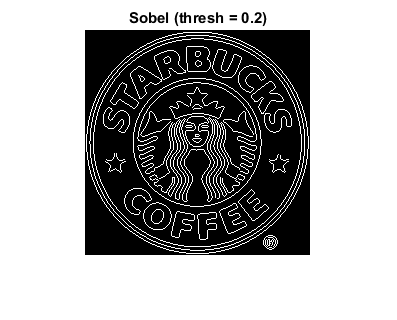
\includegraphics[width=0.6\textwidth]{3a(sobel).png}
 \end{center}
 
 - Prewitt : threshold = 0.2
 
 \begin{center}
 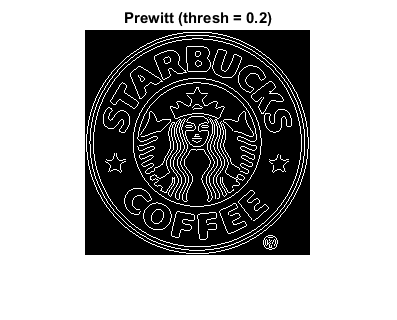
\includegraphics[width=0.6\textwidth]{3a(prewitt).png}
 \end{center} 
 
 \newpage
 - Canny : threshold = 0.1
 
 \begin{center}
 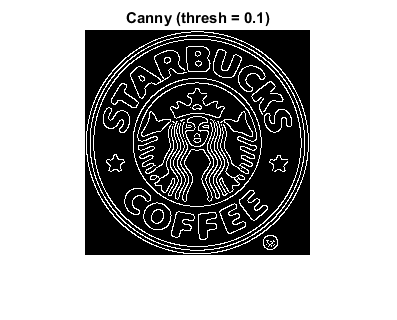
\includegraphics[width=0.6\textwidth]{3a(canny).png}
 \end{center} 
 
 - Laplaciano : threshold = 0.01

 \begin{center}
 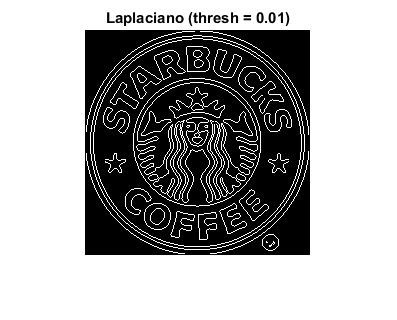
\includegraphics[width=0.6\textwidth]{3a(laplace).png}
 \end{center} 

 \newpage
 \item \textit{Repite  el  experimento  con  otras  imágenes  de  las  incluidas  en  “images.zip”. 
Comenta si los parámetros se deberían cambiar para cada imagen. }

  Cogimos la imagen coral porque es una imagen con muchos detalles y queríamos ver como se comportan los filtros en 2 casos extremos (imagen poco detallada - imagen muy detallada).

  Repetimos el experimento con los mismos threshold, excepto el de Canny, lo cambiamos a 0.15. Vimos que con estos parámetros en los filtros Sobel y Prewitt se pierde mucha información, con lo cual los parámetros deberían modificarse para adaptarlos a esta imagen.

   - Sobel : threshold = 0.2
 
 \begin{center}
 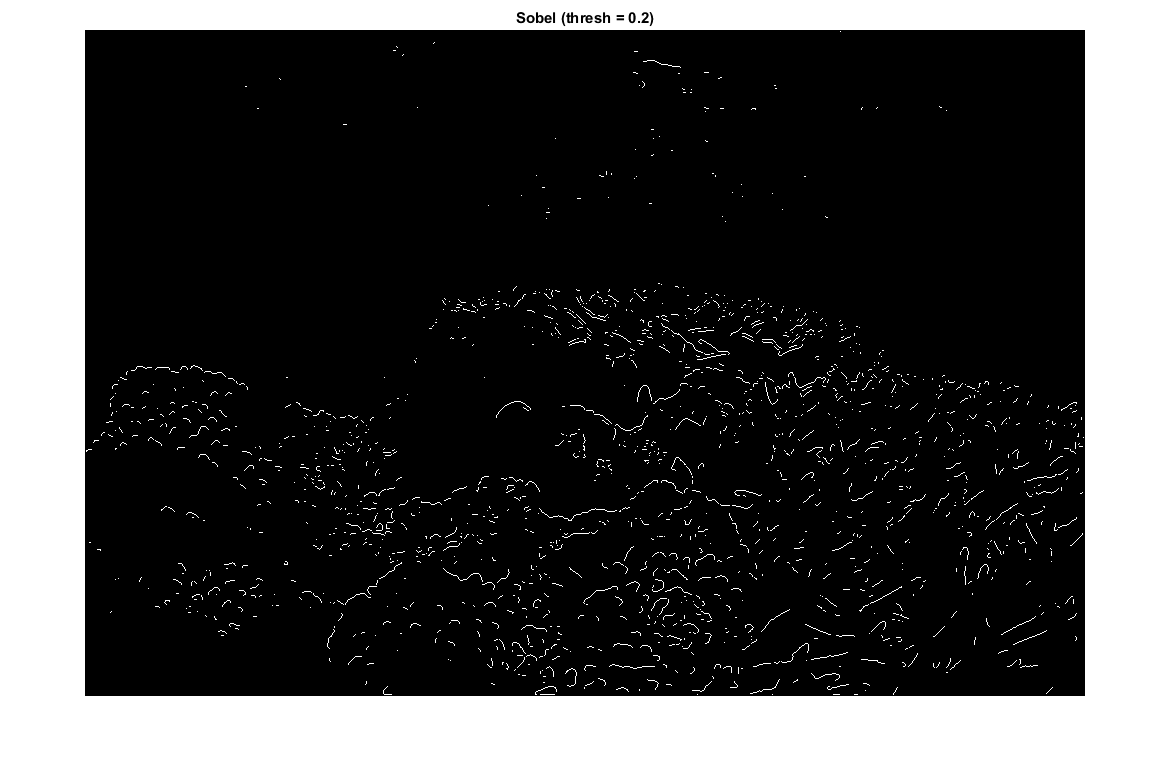
\includegraphics[width=0.6\textwidth]{3b(sobel).png}
 \end{center}
 
 - Sobel MEJORADO : threshold = 0.05
 
 \begin{center}
 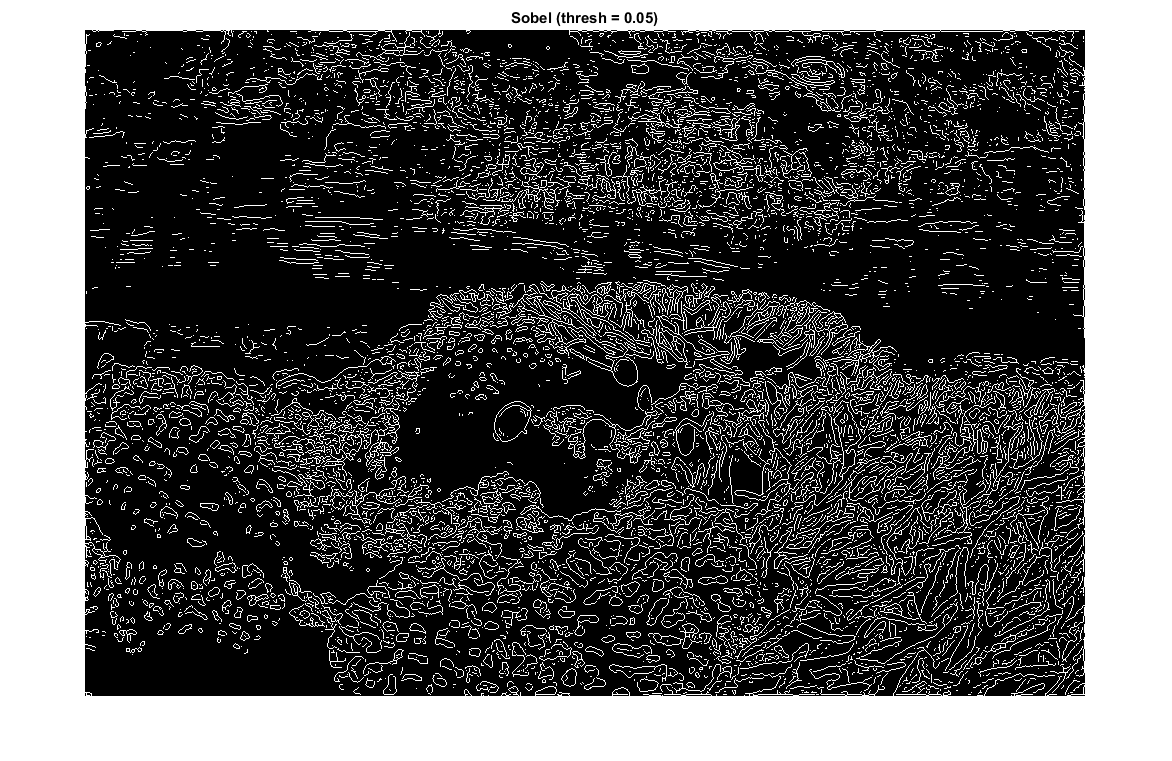
\includegraphics[width=0.6\textwidth]{3b(sobel_best).png}
 \end{center}
 
 \newpage
 
 - Prewitt : threshold = 0.2
 
 \begin{center}
 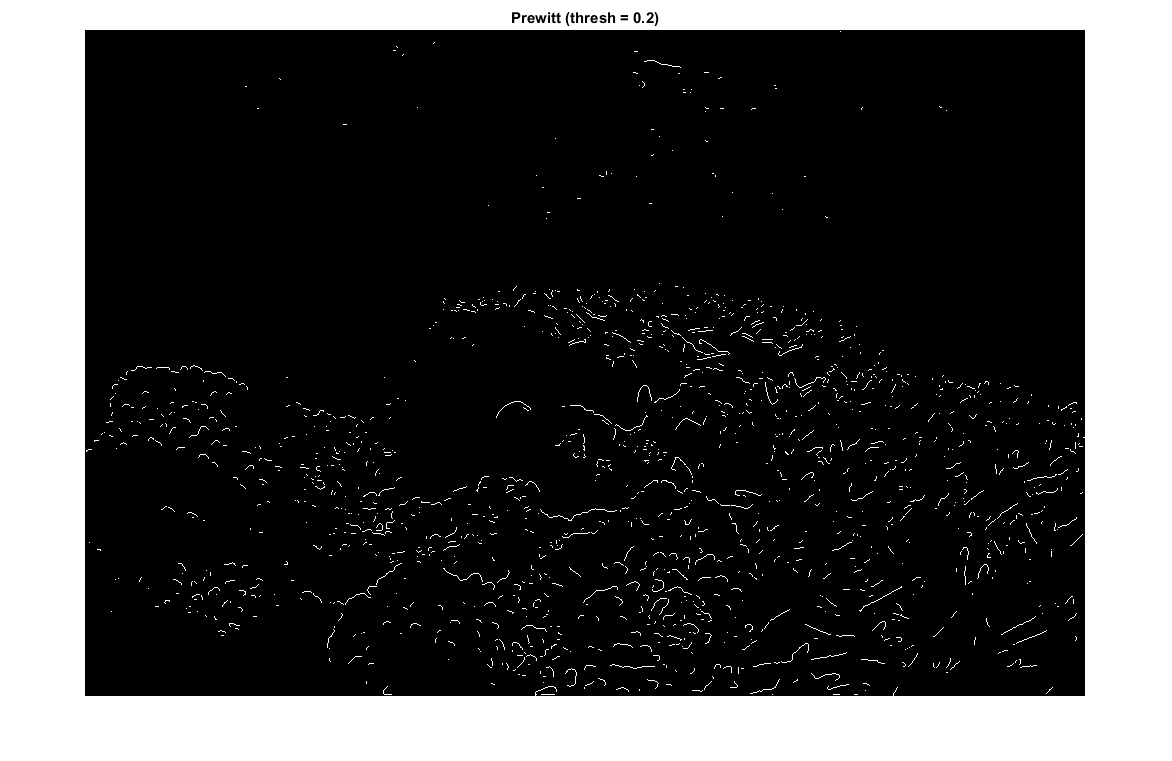
\includegraphics[width=0.6\textwidth]{3b(prewitt).png}
 \end{center} 
 
 - Prewitt MEJORADO : threshold = 0.05
 
 \begin{center}
 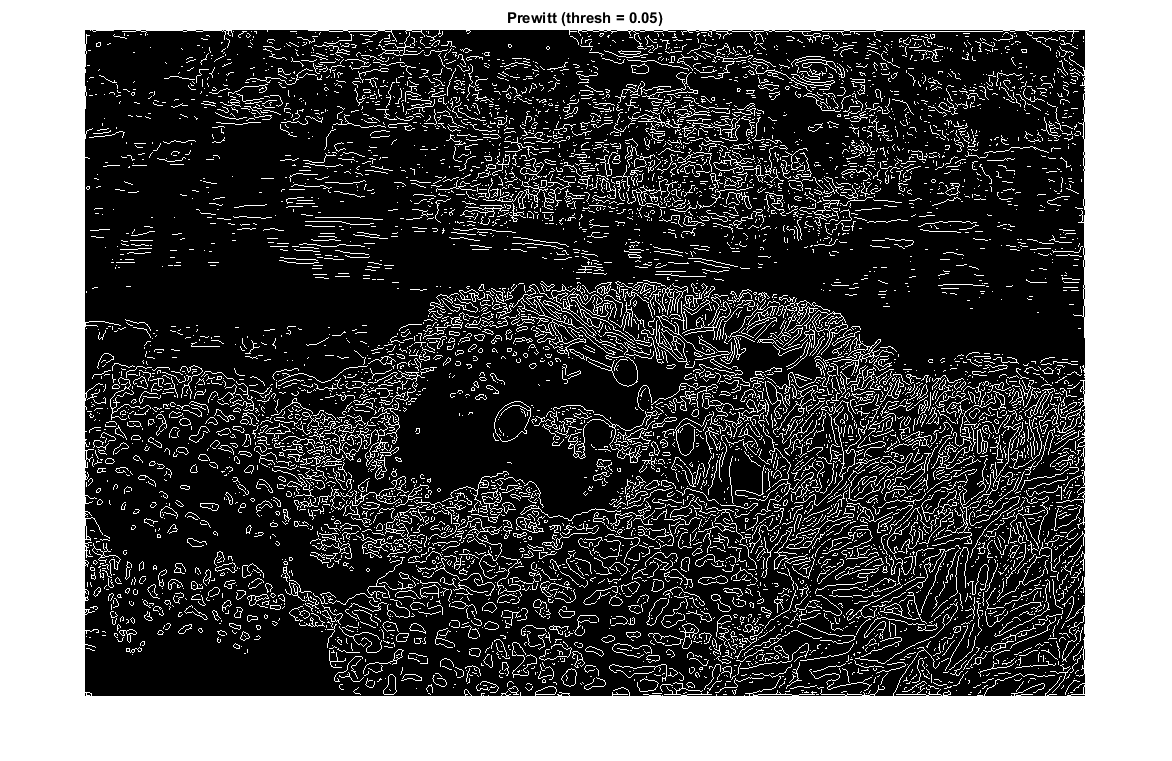
\includegraphics[width=0.6\textwidth]{3b(prewitt_best).png}
 \end{center}
 
 - Canny : threshold = 0.15
 
 \begin{center}
 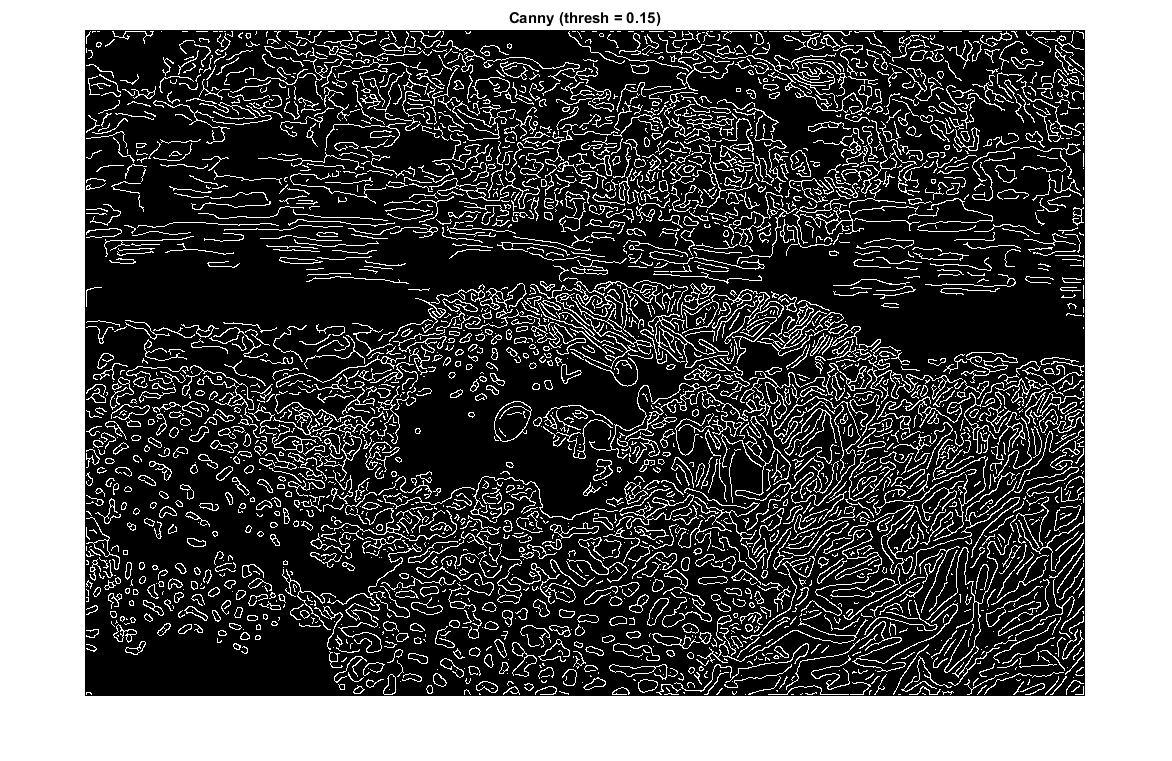
\includegraphics[width=0.6\textwidth]{3b(canny).png}
 \end{center} 
 
 \newpage
 - Laplaciano : threshold = 0.01

 \begin{center}
 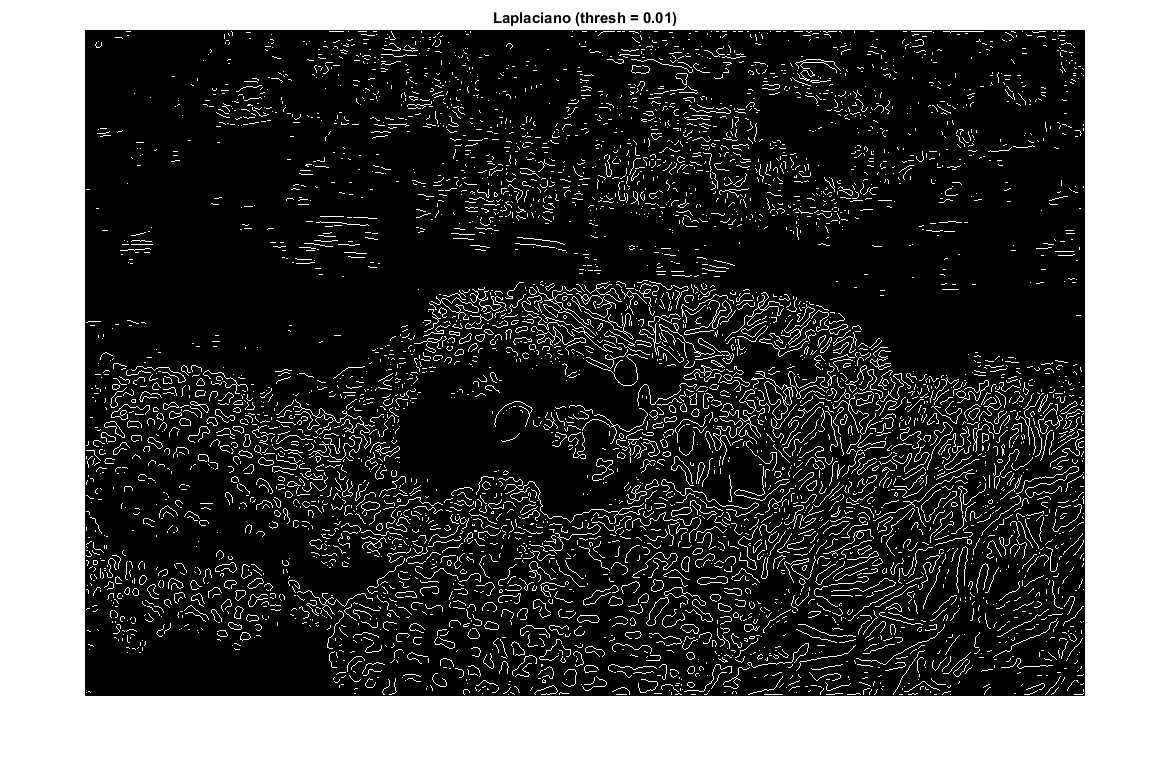
\includegraphics[width=0.6\textwidth]{3b(laplace).png}
 \end{center}
  
 \begin{enumerate} 
  \item \textit{¿Se mejoran los contornos si la imagen se suaviza antes?}
  
  A la otra imagen imagen le pasamos un filtro de la media y vimos que los contornos mejoraron, ya que suaviza las rugosidades de las texturas de los elementos de la imagen (las plantas amarillas que parecen patas de gallo, tienen las rugosidades suavizadas después del filtro que ayuda con encontrar el contorno mejor)
  
  \item \textit{¿Cuáles son las limitaciones que ves en la extracción de los contornos en las diferentes imágenes?}
  
  Habiendo hecho diferentes imágenes, vimos limitaciones como que si hay detalles relativamente pequeños (la R de copyright del de Starbucks, por ejemplo) los filtros no los detectan muy bien y si la imagen tiene muchísimos detalles es complicado ajustar los parámetros para que esos detalles se vean bien y no salga un contorno con demasiada información.
  
 \end{enumerate}
 
  
  
 \end{enumerate}

\newpage

 \item \textbf{Aplicación  de  la  suavización  para  construir imágenes híbridas} 
 
 \begin{enumerate}
 \item \textit{Dadas  las  imágenes  ‘einstein.jpg’ y  ‘monroe.jpg’,  construir  la  imagen  híbrida  y 
visualizarla a diferentes escalas para  obtener el efecto  visual de las imágenes híbridas 
(Figura 2).}  
 
 \begin{center}
 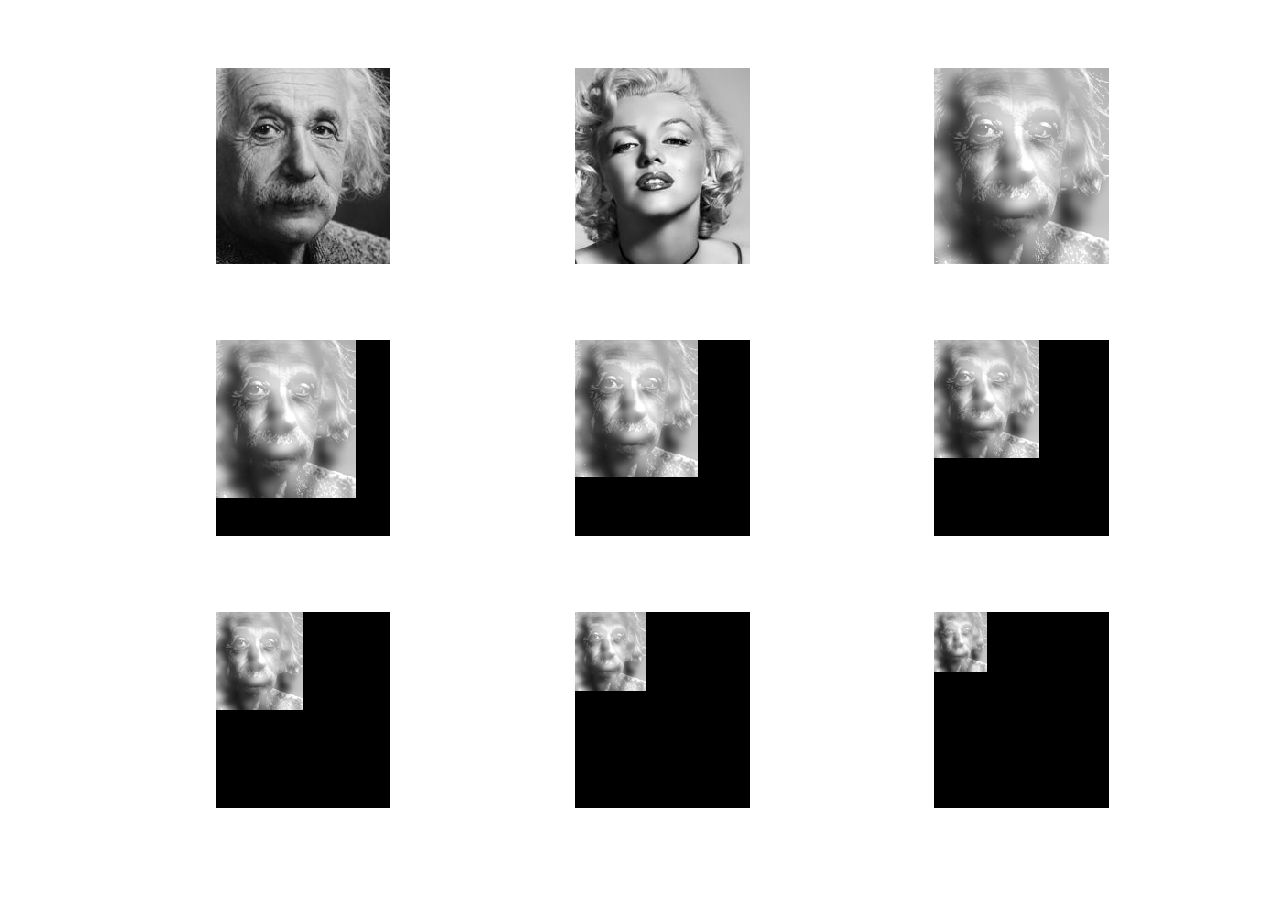
\includegraphics[width=\textwidth]{4a.png}
 \end{center}

 \item \textit{Visualizar la imagen híbrida sobre la misma figura/región para poder evaluar a partir 
de qué tamaño se pasa a percibir a  Marylin Monroe.}

  Ya está en el apartado (a)

 \end{enumerate}

\newpage

 \item \textbf{Anonimización de vídeos}

 \begin{enumerate}
 \item \textit{Dado el vídeo ‘BigBang.mp4’, filtrar las imágenes (enteras, no sólo la cara) del vídeo con la máscara adecuada (del Ejercicio 2.1) para hacer la cara no identificable. Visualizar y retornar el vídeo en color con las caras no identificables.}
 
 Usamos la máscara de gaussiano con sigma = 10. 
 
 Mostramos un frame del vídeo. El resto del vídeo después de ejecutar nuestro script de MatLab estará en el archivo "output.mp4"

 \begin{center}
 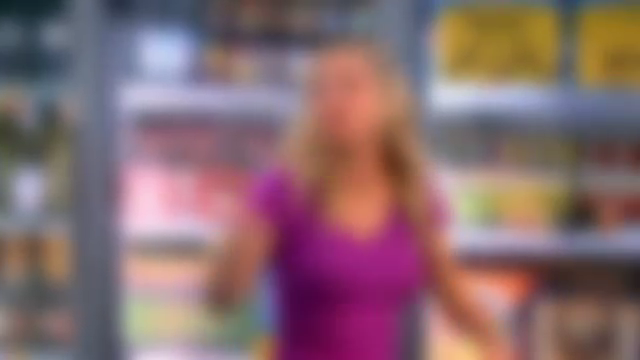
\includegraphics[width=0.6\textwidth]{5.png}
 \end{center}
 
 \end{enumerate}

\end{enumerate}

\end{document}
